\chapter{Gurobi}

\section{Introduzione a Gurobi}
L'ottimizzatore usato per la pianificazione dell'orario degli infermieri è Gurobi, che è un solutore di ottimizzazione commerciale usato in vari tipi di programmazione: lineare, quadratica, quadratica vincolata, lineare e quadratica intera mista, quadratica intera mista vincolata.

Gurobi, il cui nome deriva dai nomi dei suoi fondatori (Zonghao Gu, Edward Rothberg e Robert Bixby), è stato introdotto nel 2008 e supporta una varietà di linguaggi di programmazione e modellazione, inclusi:
\begin{itemize}
\item Interfacce Object-Oriented per C++, Java, .NET e Python;
\item Interfacce Matrix-Oriented per C, MATLAB e R;
\item Collegamenti a linguaggi di modellazione standard: AIMMS, AMPL, GAMS e MPL.
\end{itemize}

È possibile capire il ruolo di questo ottimizzatore dallo schema sottostante (Figura \ref{fig:Gurobi}).
\begin{figure}[!h]
		\centering
		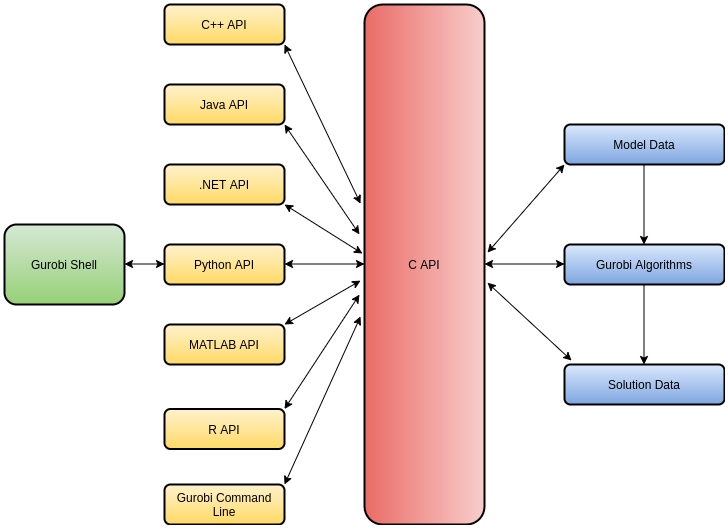
\includegraphics[scale=0.5]{img/gurobi_c.png}
		\caption{Gurobi API}
		\label{fig:Gurobi}
\end{figure}

\section{Principali API per Python}
In questa sezione vengono spiegate le funzionalità principali di Gurobi per il linguaggio Python, per dare una visione generale al lettore di come è possibile modellare un problema di ottimizzazione usando questo tipo di ottimizzatore.



\subsection{Modello}



\subsection{Variabili}
Le variabili di decisione rappresentano il risultato dell'ottimizzazione.
In una soluzione ammissibile, i valori calcolati per le variabili di decisione soddisfano tutti i vincoli del modello. Alcuni di questi vincoli sono associati a singole variabili, mentre altri rappresentano relazioni tra esse.
Ci sono varie tipologie di variabili disponibili tra cui: continue, intere o intere binarie.

%\subsubsection*{Variabili continue}
%Le variabili continue possono assumere qualsiasi valore tra il loro limite inferiore e quello superiore. Nella programmazione matematica, la convenzione è che le variabili sono non negative se non diversamente indicato, quindi se non si forniscono esplicitamente i limiti per una variabile, si dovrebbe presumere che il limite inferiore sia 0 e quello superiore sia $\infty$. Una variabile con limiti superiori e inferiori uguali ad $\infty$ vine detta variabile libera.
%Inoltre le variabili possono violare i loro limite di tolleranza, che in questo caso è \texttt{FeasibilityTol}. È possibile ridurre questo valore, ma a causa di errori numerici potrebbe non essere possibile ottenere la precisione desiderata.
%
%\subsubsection*{Variabili intere}
%Le variabili intere, in generale, sono maggiormente vincolate rispetto a quelle continue, infatti possono assumere solo valori interi. 
%
%????
%
%In particolare i limiti inferiore e superiore di una ....
%Una soluzione non è considerata ammissibile a meno che tutte le variabili 
%
%\subsubsection*{Variabili binarie}
%Le variabili binarie sono particolari variabili intere che possono assumere solo valori pari a 0 o ad 1.
%Ancora una volta, a causa dei limiti dell'aritmetica a precisione finita, le variabili binarie assumeranno spesso valori che non sono esattamente....
%L'entità della violazione di integrità consentita è controllata dal parametro \texttt{IntFeasTol}.
%
%\subsubsection*{Variabili semi-continue e semi-intere}
%Le variabili semi-continue possono assumere valori pari a 0 o ad un valore compreso tra i limiti inferiore e superiore specificati.
%Una variabile semi-intera può assumere anche un valore intero.
%
%Entrambi questi tipi di variabili possono violare queste restrizioni, in questo caso la tolleranza pertinente è \texttt{IntFeasTol}.

\subsubsection*{Metodo per aggiungere variabili al modello}
Per aggiungere una nuova variabile al modello creato è necessario usare il metodo \texttt{addVar()}, il quale se ritorna un valore diverso da 0 indica che si è verificato un problema durante l'aggiunta della variabile.
Gli argomenti che possiamo specificare in questo metodo sono:
\begin{itemize}
\item \texttt{model}: modello al quale la variabile è aggiunta;
\item \texttt{lb}: lower bound;
\item \texttt{ub}: upper bound;
\item \texttt{obj}: coefficiente obbiettivo;
\item \texttt{vtype}: tipologia della variabile in questione;
le opzioni sono:
\begin{itemize}
\item \texttt{GRB\_CONTINUOUS};
\item \texttt{GRB\_BINARY};
\item \texttt{GRB\_INTEGER};
\item \texttt{GRB\_SEMICONT};
\item \texttt{GRB\_SEMINT}.
\end{itemize}
\item \texttt{varname}: nome della variabile.
\end{itemize}

Si riporta un esempio per illustrare l'uso di questo metodo:\\
\texttt{x = model.addVar(0.0, 1.0, 0.0, GRB.BINARY, name=`x')}\\
In questo caso il primo e il secondo argomento sono, rispettivamente, il limite inferiore e superiore della variabile x. Il terzo argomento rappresenta il coefficiente di obbiettivo lineare. Successivamente viene specificato il tipo della variabile (binaria), e come ultimo argomento ne viene indicato il nome.

Nel caso si vogliano aggiungere più variabili dello stesso tipo si può usare il metodo \texttt{addVars()}.

Si noti che con entrambi questi metodi le nuove variabili non vengono effettivamente aggiunte fino a quando non si aggiorna il modello, non lo si ottimizza o non lo si  scrive su disco.

\subsection{Vincoli}
Un vincolo rappresenta una restrizione sui valori che un insieme di variabili può assumere. Vi sono varie tipologie di vincoli disponibili: lineare, quadratico, SOS, generale.

\subsubsection*{Vincoli lineari}
Un vincolo lineare consente di limitare il valore di un'espressione lineare.
Un semplice esempio può essere il seguente:
$3x + 4y ~ \leq ~ 5z$

Si noti che le API Gurobi orientate alla matrice (C, MATLAB e R) richiedono che il lato destro di un vincolo sia una costante, mentre le API orientate agli oggetti (C++, Java, .NET e Python) consentono arbitrari espressioni lineari in entrambi i membri della comparazione.

Gurobi supporta un set limitato di comparatori: in particolare, è possibile vincolare un'espressione a essere minore o uguale, maggiore o uguale o semplicemente uguale ad un'altra. Invece non vengono supportati i comparatori di minore e maggiore stretto o il comparatore di disuguaglianza. 

\subsubsection*{Vincoli SOS}
Un vincolo SOS (insieme ordinato speciale) è un vincolo altamente specializzato che pone restrizioni ai valori che possono assumere le variabili in un determinato \textbf{elenco}.
Esistono due tipi di vincoli SOS:
\begin{itemize}
\item \textit{Vincolo SOS di tipo 1}: in cui al massimo una variabile nell'elenco specificato può assumere un valore diverso da 0;
\item \textit{Vincolo SOS di tipo 2}: al massimo due variabili nell'elenco specificato e ordinato possono assumere un valore diverso da 0 e tali variabili devono essere contigue nell'elenco.
\end{itemize}
Le variabili di un vincolo SOS possono essere continue, intere o binarie.

Quindi un vincolo SOS è descritto da un elenco di variabili e un elenco di pesi corrispondenti che servono per ordinare l'elenco delle variabili in questione.

\subsubsection*{Vincoli quadratici}
Un vincolo quadratico consente di limitare il valore di un'espressione quadratica.
Un esempio è il seguente:
$3x^2 + 4y^2 + 5z ~ \leq ~ 10$.

I vincoli quadratici sono spesso molto più difficili da soddisfare rispetto a quelli lineari. ma Gurobi può gestire sia quelli convessi che non.
Tuttavia gli algoritmi predefiniti di Gurobi accettano solo alcune \textbf{forme di vincoli quadratici}, noti per avere regioni convesse realizzabili.
%come per esempio quelle elencate qui di seguito:
%\begin{itemize}
%\item $x^T Q x + q^T x ~ \leq ~ b$;
%\item $x^T x ~ \leq ~ y^2$, dove x è un vettore di variabili e y una variabile non negativa;
%\item $x^T x ~ \leq ~ y z$, dove x è un vettore di variabili, e y e z sono variabili non negative.
%\end{itemize}
%Quindi verrà accettato un vincolo quadratico solo se si è in grado di trasformarlo in una di queste forme.

Si noti che altri risolutori quadratici non convessi spesso trovano solo soluzioni localmente ottime, invece gli algoritmi su cui si basa Gurobi esplorano l'intero spazio di ricerca, quindi forniscono un limite inferiore valido a livello globale e quindi, dato un tempo sufficiente, potranno trovare una soluzione ottima globale.

\subsubsection*{Vincoli generali}
I vincoli sopra descritti sono generalmente gestiti direttamente dagli algoritmi di ottimizzazione sottostanti. Gurobi include una serie aggiuntiva di vincoli, chiamati vincoli generali, progettati per una questione di praticità e funzionalità, in quanto permettono di definire facilmente determinate relazioni variabili.

Vi sono due tipologie di vincoli generali:
\begin{itemize}
\item \textit{Vincoli di funzione}, come per esempio $y ~ = ~ f(x)$, dove $x$ e $y$ sono due variabili decisionali e $f()$ è la funzione scelta in una lista di funzioni tra le seguenti: polinomiale, esponenziale, logaritmica, potenza, seno, coseno e tangente;
\item \textit{Vincoli semplici generali}, che consentono di stabilire relazioni comuni ma più dirette tra le variabili decisionali, e quelli supportati da Gurobi sono:
\begin{itemize}
\item vincolo \texttt{MAX}
\item vincolo \texttt{MIN}
\item vincolo \texttt{ABS}
\item vincolo \texttt{AND}
\item vincolo \texttt{OR}
\item vincolo \texttt{INDICATOR}
\item vincolo lineare a tratti
\end{itemize}
\end{itemize}

\subsubsection*{Metodo per aggiungere vincoli al modello}
Per aggiungere un nuovo vincolo al modello preso in esame viene usato il metodo \texttt{addConstr()}, dove i principali argomenti che accetta sono:
\begin{itemize}
\item \texttt{lhs}: membro sinistro del vincolo;
\item \texttt{rhs}: membro destro del vincolo;
\item \texttt{sense}: senso del vincolo, che può essere:
\begin{itemize}
\item \texttt{GRB.EQUAL};
\item \texttt{GRB.LESS\_EQUAL};
\item \texttt{GRB.GREATER\_EQUAL}.
\end{itemize}
\item \texttt{name}: nome de nuovo vincolo.
\end{itemize}

Un esempio dell'utilizzo di questo metodo è il seguente:\\
\texttt{model.addConstr(x + 2y, GRB.EQUAL, 3Z, name=`C\_0')}

\subsection{Funzione obbiettivo}
Ogni modello di ottimizzazione ha una funzione obbiettivo, che è la funzione definita mediante le variabili decisionali che si desidera minimizzare o massimizzare.
La maggior parte dei problemi ha molteplici soluzioni ottimali, quella restituita da Gurobi dipende dal tipo di problema preso in esame.
In generale questo ottimizzatore restituisce un'unica soluzione ottimale per modelli continui e una sequenza di soluzioni migliorative per modelli discreti.

Gli algoritmi di Gurobi lavorano per risolvere un modello fino a quando non trovano una soluzione ottimale entro le tolleranze specificate.
Per modelli discreti, nonostante sia possibile chiedere al risolutore di trovare una soluzione con il miglior valore obbiettivo, è molto comune fermarsi quando l'obbiettivo della soluzione rientra in un intervallo specificato del valore ottimale.
Questo Gap dell'ottimalità è controllato dal parametro \texttt{MIPGap} il cui valore predefinito è 0,01\%.

Le funzioni obbiettivo possono essere: lineari, quadratiche, lineare a tratti e multi-obbiettivo lineari.

\subsubsection*{Metodi principali della funzione obbiettivo}
Per impostare l'obbiettivo del modello uguale ad un'espressione lineare o quadratica viene usato il metodo \texttt{setObjective()}, che ha come parametri:
\begin{itemize}
\item \texttt{linExpr} o \texttt{quadExpr}: espressione lineare o quadratica:
\item \texttt{sense}: si può specificare se si desidera minimizzarla o massimizzarla.
\end{itemize}

Per esempio sia $f(x)$ la funzione obbiettivo, supponiamo di volerla minimizzare:\\
\texttt{model.setObjective($f(x)$, GRB.MINIMIZE)}\\
Una volta settata la funzione obbittivo per minimizzarla è necessario richiamare il metodo \texttt{optimize()} sul modello in questione:\\
\texttt{model.optimize()}